\documentclass{amia}
\usepackage{graphicx}
\usepackage[labelfont=bf]{caption}
\usepackage[superscript,nomove]{cite}
\usepackage{color}
\usepackage{multirow}


\begin{document}


\title{Sequence classifications to facilitate designing an effective intervention of motivational interview}

\author{Mehedi Hasan, BS$^{1}$, Alexander Kotov, PhD$^{1}$, April Carcone, PhD$^{2}$, Sylvie Naar-King, PhD$^{2}$}

\institutes{
$^1$Department of Computer Science,  
$^2$Pediatric Prevention Research Center, Wayne State University, Detroit, Michigan\\
}

\maketitle

\noindent{\bf Abstract}
\textit{Childhood obesity is a serious public health concern in the United States and worldwide. Therefore, there is a need for identification of successful motivational interviews to facilitate the development of effective interventions for childhood obesity. This paper presents our work on the classification of utterance sequences into successful and unsuccessful behavior outcomes. Markov chain and hidden Markov models were employed and compared with a different order for the classification of utterance sequences. The classification performances achieved 75.32\% and 79.89\% F-measure for normal sequences and 97.36\% and 96.99\% F-measure for alternate sequences using 1st order Markov chain and second order hidden Markov model, respectively. This shows that the behavior codes carry some inherited information to distinguish motivational interviews. We expect that the result will improve if we use a more discriminable data set. Furthermore, the results suggest us a new way to think about designing the motivational interview.}

\section*{Introduction}
In the recent times, more and more data from various domains being produced in the form of event sequences. Thus, sequence classification has become an important task in sequence mining. Sequences can contain discrete (e.g., symbolic sequences such as text, proteins, or DNA) or continuous events (e..g, time series such as ECGs or stocks), depending on the event types. Usually, sequences don't have explicit features and suffer from the high dimension of feature space. Even the sequential nature of features is too difficult to capture, which make sequence classification, a more challenging task than feature-based classifications. The sequence classification methods can be divided into three large categories: feature-based classification, distance based method, and model based classifications. In feature-based classification, a sequence is transformed into a single vector of features. A supervised learning algorithm such as a support vector machine \cite{leslie2004fast} or decision tree \cite{chuzhanova1998feature} can be used to train the classifier. An improvement of feature-based classifier such as shapelet \cite{ye2009time} or pattern-based \cite{kudenko1998feature, lesh1999mining} approach is used for sequence classifications. On the other hand, distance based method measure the similarity between sequences to determine the quality of the classification significance. The most commonly used distance function is euclidian distance \cite{keogh2003need}, while Dynamic Time Wrapping \cite{keogh2000scaling} is used when more flexible matching is desired in time series data. The third category of sequence classification is model based classifiers such as hidden Markov model \cite{rabiner1989tutorial} (HMM) or other statistical models. Recently, a hierarchical approach \cite{nallam2016effective} is proposed for sequence classification. 

Sequence classification has a broad range of real word applications such as information retrieval, genomic analysis, health informatics, finance and abnormal detection. In genomic research, sequence classification is widely used to detect the function of a new protein \cite{deshpande2002evaluation}. In health informatics, ECG can be used as a multi-dimensional time series data to classify an individual as healthy or patient with heart disease \cite{wei2006semi}. Another example is to classify rumor stance in Twitter \cite{lukasik2016hawkes}. In information retrieval, sequence classification is employed to build models for classifying documents into different topic categories \cite{sebastiani2002machine} such as sports, politics, news, finance and style. Sequence classification is also used in anomaly detection such as abnormal access to systems \cite{lane1999temporal}, malware detection \cite{drew2017polymorphic} and money laundering \cite{liu2008sequence}. Other interesting applications include classifying query log sequences to distinguish web-robots from human users \cite{duskin2009distinguishing, tan2004discovery}. In computer vision, sequence classification is applied for classifying images \cite{li2000image} and videos \cite{zhang2016tensor}.    

In this paper, our target area of application is the motivational interview. In particular, this paper describes our work on the classification of utterance sequences. Classification of utterance sequences to distinguish different behavior outcomes such as positive change talk or commitment versus negative change talk or commitment is an important part of clinical research aimed at designing effective interventions for many conditions and disorders. In this study, we focus on the transcripts of Motivational Interviews (MI) with obese adolescents (teens) and their caregivers. Childhood obesity is a serious public health concern in the United States and worldwide. Recent estimates indicate that approximately one third (31.8\%) of US children age 2-19 years are overweight and 16.9\% are obese \cite{ogden2012prevalence}. Adolescents who are obese likely continue to be obese in adulthood and have a greater risk of heart disease, type 2 diabetes, stroke, cancer, and osteoarthritis \cite{general2010surgeon}. Therefore, there is a need for informatics-based methods to facilitate the development of effective interventions for childhood obesity. One approach to designing an effective intervention is Motivational Interviewing, an evidence-based counseling technique to increase intrinsic motivation and self-efficacy for health-related behavior change. The goal of MI counseling session is to encourage patients to explore their own desires, ability, reasons, need for and commitment to the targeted behavior change. These statements, referred to as ``change talk'' (or CT), consistently predict actual behavior change that can be sustained for as long as 34 months after an interview. 

Our previous studies \cite{kotov2015interpretable, hasan2016study} explored several machine learning methods for the automatic annotation of clinical interview fragments, which uses a codebook \cite{carcone2013provider} with 115 different behavior codes. In this study, probabilistic models are employed for the analysis of sequence data to determine provider-patient communication sequences that are likely to translate into change talk and commitment language. To the best of our knowledge, there have been very limited studies on sequence classification in a motivational interview such as patient-provider dialogue. A sequential analysis \cite{eide2004physician} was performed on physician-patient dialogue to find the relationship between physician and patient behaviors associated with patients' exhibiting cues. Currently, a very similar work \cite{jaber2016multi} was done on education data, where a sequence classification model was developed to predict the role of a student in a project team based on their communication patterns. Although hidden Markov model was originally applied to speech recognition \cite{rabiner1989tutorial}, this is one of the most successful method \cite{mutsam2016maximum, eickeler1998hidden, srivastava2007hmm, won2004training, chai2001folk} for sequence classification. In addition, a k-order Markov model is applied to genomic research \cite{yakhnenko2005discriminatively} to classify protein and text sequence data. Therefore, we utilize Markov chain and hidden Markov model for the classification of utterance sequences. 

\section*{Methods}
\subsection*{\textit{Data collection}}
The experimental data sets for this work were constructed based on the transcripts of 37 motivational interview sessions, which include a total of 11,353 segmented and annotated utterances. Since clinical researchers tried to increase the desire and ability of an adolescent to change their current behavior to target behavior, we used sequences from an adolescent session and excluded sequences from caregiver session in the MI transcript. The utterances were annotated based on MYSCOPE codebook \cite{carcone2013provider} with 115 different behavior codes, which are grouped into the youth, caregiver, and counselor code groups. These utterances are then scanned from first to last and divided into successful and unsuccessful sequences when a commitment or change talk is found. A total of 1072 sequences have been observed which further partitioned into two subsets based on the outcome of motivational interviews: one data set that includes all sequences of positive change talk or commitment language (880 sequences) and the other data set which includes utterances ended with negative change talk or commitment language (192 sequences). Alternate sequences are the possible combination of a normal sequence where two consecutive codes can not come from the same speaker. For example, there are 6 possible alternate sequences for the following sequences: (C1, A1, A2, C2, C3, C4, A3), where adolescent and counselor codes are represented by A and C, respectively. Therefore, (C1, A1, C2, A3), (C1, A1, C3, A3), (C1, A1, C4, A3), (C1, A2, C2, A3), (C1, A2, C3, A3) and (C1, A2, C4, A3) were used as alternate sequences for the above sequence. A total of 18753 alternate sequences has been observed which further partitioned into two subsets of 18139 successful and 614 unsuccessful sequences. In our experiment, normal and alternate sequences are employed with two subsets (successful and unsuccessful) to train Markov chain and HMM. Dataset statistics and a fragment of an adolescent session transcript are presented in Table~\ref{tab:data_dist} and Table~\ref{tab:anno_examp}. \\

\begin{table}[h]
\centering
\caption{General statistics of dataset.}
\label{tab:data_dist}
  \begin{tabular}{|l|l|l|l|l|l|}
  \hline
   \textbf{Sequence type} & \textbf{Total sequences}  & \textbf{\# Successful sequences}  & \textbf{\# Unsuccessful sequences} & \textbf{Avg. length} \\ \hline      
 Normal sequences & 1072 & 880 (82.09\%) & 192 (17.91\%) & 5.83 \\\hline
Alternate sequences & 18753 & 18139 (96.72\%) & 614 (3.28\%) & 12.89 \\\hline 
  \end{tabular}
\end{table} 

Annotation column in Table~\ref{tab:anno_examp} shows the sequence of behavior codes from top to bottom, where counselor start with an open-ended question and get positive feedback at the end. \\

\begin{table}[h]
\caption{Fragment of the annotated transcript of a dialogue between a counselor and an adolescent.}    
\label{tab:anno_examp}
\centering
\begin{tabular}{|l|p{3.6cm}|l|p{8cm}|}
\hline
Annotation  & Description & Speaker & Text \\\hline
331 &	Open-ended question, elicit change talk positive &	Counselor &	do you feel like making healthier choices for your snacks and your meals is something you would be able to do? mm-hmm meaning is that food available for you? \\\hline
117 &	Low Uptake, positive	& Adolescent &	Yes \\\hline
301 &	Structure Session	& Counselor &	okay and thats an important thing for us to think about cause i would not want to help you come up with a plan that you would not be able to do without somebody else help so the last part of your plan is how somebody could be supportive to you meaning how they can help you be successful and so we should choose somebody who you feel like is around often enough \\\hline
112 &	Change Talk positive	& Adolescent &	my um aunt \\\hline
301 &	Structure Session	& Counselor &	okay so lets stick something my aunt can do \\\hline
112 &	Change Talk positive &	Adolescent &	she could when i am doing when i am eating something that i should i could not be eating but so i can choose something healthy she could tell me not to eat it \\\hline
309 &	Affirm, low &	Counselor &	okay that sounds like a really great suggestion \\\hline
\end{tabular}
\end{table}  

\subsection*{\textit{Sequence classification techniques}}
Generally, a sequence is an ordered list of events. In our study, an event is a behavior code represented as a symbolic value such as 117 (low uptake, positive), 331 (open-ended question), etc.  Given a sequence of behavior codes represented as $S_i = \{x_1, x_2,...,x_n\}$ and a set of class labels $L = \{l_1, l_2,...,l_m\}$, the task of sequence classification is to learn a sequence classifier C, which is a function mapping a sequence $S_i$ to a class label $l_i \in L$, written as, $C : S_i \to l_i, l_i \in L$. Here, L is fixed and known in advances. In our experiment, known labels are ``successful'' and ``unsuccessful'' motivational interview. 

\textbf {Markov Chain}: In probability theory, a Markov model \cite{} is a stochastic model used to model randomly changing systems where it is assumed that future states depend only on the present state and not on the sequence of events that preceded it (that is, it assumes the Markov property). Generally, this assumption enables reasoning and computation with the model that would otherwise be intractable. For the sequential analysis, we built two Markov models $M$ and $\overline{M}$ describing provider strategies and patient responses in case of successful ($M$) and unsuccessful ($\overline{M}$) motivational interviews. A Markov model $M$ can be represented as a weighted directed graph $G = (V, E, p)$, in which:

\begin{itemize}
\item $V = \{CML+, CHT+, CHT-, T-AMB, CCT, BLT, LUP+, LUP-, HUP-W, ...\}$ is a set of vertices, consisting of possible youth and counselor MI behavior codes;
\item $E \subseteq V \times V$ is a set of edges corresponding to posssible transitions from one MI behavior code to the other in a sequence;
\item $p_M:E\rightarrow[0...1]$ is a function that assigns probability $p(c_i|c_j)$ to an edge between the MI behavior codes $c_i$ and $c_j$ based on maximum likelihood estimator:

\begin{equation}
P_M(c_j|c_i) = \frac{n_{c_i,c_j}}{n_{c_i}}
\end{equation}

\end{itemize}

where $n_{c_i,c_j}$ and $n_{c_i}$ are the number of times a transition between the MI behavior codes $c_i$ and $c_j$ and the code $c_i$ have been observed in the training data. Given a Markov model $M$ (such that $S\subseteq V$), a sequence of MI behavior codes $S = \{C_1,...,C_N\}$ have been generated from a Markov model $M$ is:

\begin{equation}
P_M(S) = \prod_{i=2}^N p_M(c_i|c_1,\dots,c_{i-1})=\prod_{i=2}^N p_M(c_i|c_{i-1})
\end{equation}

Success of a given motivational interview, given a sequence of MI behavior codes corresponding to it, can be predicted based on the following formula:

\begin{equation}
p(S\rightarrow CML+) = \log\left(\frac{P_M(S)}{P_{\overline M}(S)}\right)= \sum_{i=2}^N p_M(c_i|c_{i-1})-\sum_{i=2}^N p_{\overline M}(c_i|c_{i-1})
\end{equation}

if $p(S\rightarrow CML+) > \delta $, where $\delta$ is experimentally defined threshold, the interview transcript (or a portion of it) is predicted to result in positive commitment. To fit the model, we experimentally determined the value of $\delta$ where model provides highest F-measure with lower bias. Figure~\ref{fig:delta} illustrates an example of the characteristics of Markov model by varying the value of $\delta$. From the figure, it was observed that F-score value is not changing significantly with respect to $\delta $ from -5 to -1. This is because a bias is involved. However, F-score sharply decreased after $\delta = -0.9$. Thus, -0.9 will be the optimal value of $\delta $, where F-measure is highest with lower bias. 

\begin{figure}[htb!]
    \centering
    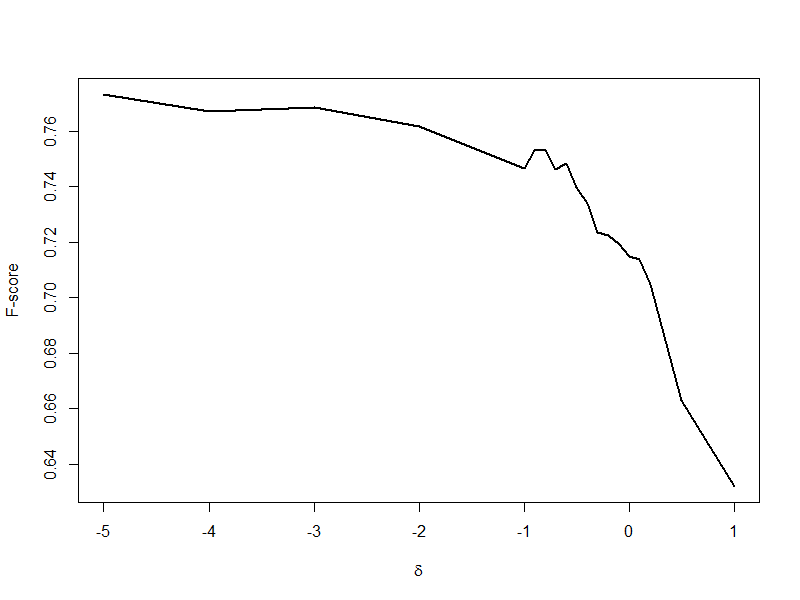
\includegraphics[width=0.70\textwidth]{figures/delta.png}
    \caption{\textbf{Characteristics of proposed Markov model by varying the value of $\delta$}}
    \label{fig:delta}
\end{figure}

The Markov model we have discussed so far is referred to as the first-order Markov model, since we only look one code in the past to compute the transition probability. A generalization of the first-order Markov model is the $k^{th}$ order Markov chain in which the transition probability for a particular symbol $x_i$ is computed by looking at the k preceding symbols. Thus, $k^{th}$ order Markov chain will have $N^{k}$ states each associated with a sequence of k symbols. In our experiment, we also used second order Markov model. Hence, our model has $N^2$ states with transitional probability matrix of size $N^2 \times N$.  

\textbf {Hidden Markov Model (HMM)}: hidden Markov models are widely used for sequence analysis because of their ability to incorporate dependencies among elements in sequence. Hidden Markov model is a very
powerful tool to statistically model a process that varies in time. It can be seen as a doubly embedded stochastic process with a process that is not observable (hidden process) and can only be observed through another stochastic process (observable process) that produces the time set of observations. An HMM can be fully specified by the following quintuple:

\begin{center}
$\lambda = (N, M, A, B, \pi)$
\end{center}

\begin{itemize}
\item N is the number of states for the model
\item M is the number of distinct observations symbols per state, i.e. the discrete alphabet size
\item A is the $N\times N$ state transition probability distribution given in the form of a matrix $A = \{a_{ij}\}$
\item B is the $N\times M$ observation symbol probability distribution given in the form of a matrix $B = \{b_j(k)\}$
\item $\pi$ is the initial state distribution vector $\pi = \{\pi_i\}$
\end{itemize}

If we opt out the structure parameters M and N we have the more often used compact notation:

\begin{center}
$\lambda = (A, B, \pi)$
\end{center} 

This model is also called hidden for a reason. We are not required to tell it what those aforementioned states should be. We just have to tell it how many states we think are needed to model what we want. The model should be able to figure a suitable sequence of states to support our observations. The Baum-Welch algorithm was implemented to train a hidden Markov model for estimating parameters of each models using the training set. To identify the label of an unknown code sequence, the Viterbi algorithm was used to decode the sequence and compute its log probabilities respectively using HMM's trained for different classes. Then, the class with the highest log probability was assigned to the given behavior sequences. Like Markov chain, we also employed second order hidden Markov model for classification of utterance sequences.   

\subsection*{\textit{Evaluation methods}}
The performance of classifiers is reported on the basis of 5-fold cross-validation by using weighted macro-averaging over folds. Precision, recall, F-measure and accuracy were used to evaluate the performance of classifiers. A true positive (TP) was counted when classifier correctly classified the sequence into actual class; a false positive (FP) was counted when classifier incorrectly classified other classes to the considered class; a false negative (FN) when the considered class incorrectly classified to other classes. The precision of a class was defined as the ratio between the numbers of correctly classified sequences and all sequences identified as that particular class by the classifier. In other words, Precision = TP / (TP + FP). Recall of a class was defined as the ratio between the numbers of correctly classified sequences and all sequences of that particular class in the gold standard (labeled data set). In more specifically, Recall = TP / (TP + FN). Similarly, Accuracy of a class was also defined as the ratio between the numbers of correctly classified sequences and a total number of sequences for that particular class in the gold standard. However, F-measure can be computed as the harmonic mean of precision and recall, or 2 x Precision x Recall / (Precision + Recall).  

\section*{Results}
Experimental evaluation of the classification of utterance sequences by using probabilistic models is reported with two set of experiments: the first set of experiment was focused on normal sequences, while the second set of experiment was performed on alternate sequences. 

\subsection*{\textit{Performance of models for the classification of normal PPC code sequences}}
Performance summary for the classification of normal sequences is presented in Table~\ref{tab:result_norm_seq}. It follows that first order hidden Markov model works very well and achieves highest precision 0.7980 with F-measure 0.7989. However, our designed second order Markov model shows the lowest performance in terms of precision and F-measure. It was also noticed that the lowest recall 0.7686 achieved in first order Markov model. On the other hand, second order hidden Markov model achieves the highest recall 0.8449 and accuracy 0.8449. From Table~\ref{tab:result_norm_seq}, we observed that performance degrades from first order to second order. Precision and F-measures drop 6.74\% \& 2.39\% in Markov chain and 7.27\% \& 2.09\% in HMM, respectively, when using second order models. In contrast, recall improves 2.64\%--4.84\% in second order Markov model and HMM. Overall, HMM performed better than general Markov model in normal utterance sequences. \\

\begin{table}[h]
\centering
\caption{Performance of Markov models for the classification of normal PPC code sequence. Highest performances for each metrics are highlighted in bold faces.}
\label{tab:result_norm_seq}
  \begin{tabular}{|l|l|l|l|l|l|}
  \hline
   \textbf{Model} & \textbf{Order}  & \textbf{Precision}  & \textbf{Recall} & \textbf{F-Measure} & \textbf{Accuracy}\\ \hline    
    
 \multirow{2}{*}{General Markov chain} & First order & 0.7387 & 0.7686 & 0.7532 & 0.7686\\\cline{2-6}
 & Second order & 0.6889 & 0.7889 & 0.7352 & 0.7889\\ \hline
 \multirow{2}{*}{Hidden Markov Model} & First order & \textbf{0.7980} & 0.8059 & \textbf{0.7989} & 0.8059\\ \cline{2-6}
 & Second order & 0.7400 & \textbf{0.8449} & 0.7822  & \textbf{0.8449}\\ \hline
 
  \end{tabular}
\end{table} 

\subsection*{\textit{Performance of models for the classification of alternate PPC code sequences}}
Table~\ref{tab:result_alt_seq} shows the classification performance of models applied on alternate sequences. The results demonstrate that second order hidden Markov model performed better than Markov chain in terms of recall and achieved 97.13\% recall. Second order general Markov model shows the highest precision 0.9778 as well as highest F-measure 0.9736. On the other hand, first order hidden Markov model displays the lowest performance in all metrics compared to all other models. It was also examined that every model perform better in second order compared to first order. General Markov chain achieves 0.01\%, 2.72\% and 1.37\% improvement for precision, recall and F-measure, respectively, from first order to second order. Similarly, hidden Markov model achieves 3.32\%, 4.30\% and 4.82\% improvement for precision, recall and F-measure, respectively, from first order to second order. Overall, second order Markov model performs better for alternate utterance sequences. \\

\begin{table}[h]
\centering
\caption{Performance of Markov models for the classification of alternate PPC code sequence. Highest performances for each metrics are highlighted in bold faces.}
\label{tab:result_alt_seq}
  \begin{tabular}{|l|l|l|l|l|l|}
  \hline
   \textbf{Model} & \textbf{Order}  & \textbf{Precision}  & \textbf{Recall} & \textbf{F-Measure} & \textbf{Accuracy}\\ \hline    
    
 \multirow{2}{*}{General Markov chain} & First order & 0.9777 & 0.9437 & 0.9604 & 0.9437\\\cline{2-6}
 & Second order & \textbf{0.9778} & 0.9694 & \textbf{0.9736} & 0.9694\\ \hline
 \multirow{2}{*}{Hidden Markov Model} & First order & 0.9392 & 0.9313 & 0.9253 & 0.9392\\ \cline{2-6}
 & Second order & 0.9704 & \textbf{0.9713} & 0.9699  & \textbf{0.9713}\\ \hline
 
  \end{tabular}
\end{table}

\subsection*{\textit{Some common patterns}}
Table~\ref{tab:common_patterns} shows some successful and unsuccessful patterns which appeared more frequently in a motivational interview. It can be seen that most successful patterns start with a summary of the discussion or open-ended or closed-ended question. After that, if adolescent demonstrates positive behavior change, counselor reflect that positive attitude immediately so that adolescent can stick with the decision and show his own desire for positive behavior change. On the other hand, general information of counselor can lead to a negative behavior change of adolescent, while showing a positive attitude in the previous step. Because adolescent changes their topic more frequently when general questions were asked.   

\begin{table}[h]
\centering
\caption{Some common patterns in motivational interview for successful and unsuccessful behavior outcome.}
\label{tab:common_patterns}
  \begin{tabular}{|l|l|l|l|l|l|}
  \hline
   \textbf{Type} & \textbf{Pattern} \\ \hline      
successful & 328 SUM-S: Summarize $\rightarrow $ 117 LUP+: Low Uptake, positive $\rightarrow $ 313 R-CML+: Reflect, \\ 
& commitment language positive $\rightarrow $ [positive commitment] \\\hline
successful & 307 SPT: Support $\rightarrow $ 117 LUP+: Low Uptake, positive $\rightarrow $ 313 R-CML+: Reflect, \\
& commitment language positive $\rightarrow $ [positive commitment] \\\hline
successful & 306 CQ-EF: Closed question, Elicit Feedback $\rightarrow $ 120 HUP-O: High Uptake, other \\
& $\rightarrow $ 313 R-CML+: Reflect, commitment language positive $\rightarrow $ [positive commitment] \\\hline
unsuccessful & 311 R-CT+: Reflect, change talk positive $\rightarrow $ 117 LUP+: Low Uptake, positive $\rightarrow $ 302 G-INFO+:  \\
& General Information, positive $\rightarrow $ [negative commitment] \\\hline
unsuccessful & 302 G-INFO+: General Information, positive $\rightarrow $ 117 LUP+: Low Uptake, positive $\rightarrow $  \\
& 302 G-INFO+: General Information, positive $\rightarrow $ [negative commitment] \\\hline
unsuccessful & 305 EA: Emphasize Autonomy $\rightarrow $ 117 LUP+: Low Uptake, positive $\rightarrow $ 302 G-INFO+:  \\
& General Information, positive $\rightarrow $ [negative commitment] \\\hline
  \end{tabular}
\end{table} 

\section*{Discussion}
The purpose of this study was to facilitate the design of motivational interview by examining the performance of sequence classification in the field of health informatics. Studying the results across the different classification schemes we can make some key observations. 

First, higher order models have better classification accuracy as compared to lower order models because they are able to capture longer ordering constraints present in the data set. However, the number of states in higher order Markov chains grows exponentially with the order of the chain. Consequently, it is harder to accurately estimate all the transition probabilities from the training set. That is, there are many high-order states that are not frequently observed in the training set, leading to inaccurate probability estimates. In principle, this problem can be solved if the size of the training set is increased at the same rate as the state-size of the higher order Markov chain. However, this cannot be easily done for many applications areas include our case. To skip these problems we restricted our study up to second order. The shorter average length of utterance sequence is another reason for keeping the order lower.  

Second, the overall accuracy of hidden Markov model is better than general Markov model in both types of sequences. We observed that hidden Markov model achieved near-human accuracy to categories the sequences of behavior codes. This means that hidden states capture the information passes through the codes of the utterance sequence for determining the final outcome. 

Third, alternate sequences provide higher performance for all Markov models. Even it provides the highest precision and F-measure for general Markov model. This indicates that each pair of alternate behavior codes forward their mutual information to the next step more accurately which improve performance for distinguishing outcomes of the motivational interview. And this is obvious because if we know the previous two behavior codes, for instance, provider's question and adolescent's response then it is easier to know the expected response for the current question of the counselor.   

Finally, it was seen that successful interviews are more frequently responded by the adolescent with positive behavior changes which lead to making a positive commitment for loosing weight. Whereas, unsuccessful interviews are responded with negative behavior changes which lead to a negative commitment or no commitment. 

\section*{Conclusion}
It has been shown how Markov chain and hidden Markov models could be used to build classifiers for the sequence of behavior codes in motivational interviews. Experimental results show that the behavior codes carry some inherited information to distinguish motivational interviews. This work can facilitate researchers to establish a causal relationship between different communication strategies and desired behavioral outcomes without having to repeatedly wade through pages of interview transcripts. It provides information that can directly inform and increase the efficiency of clinical practice for a successful interview. This work also explains some successful patterns for the practical use by the clinician during the interview session which will translate into positive change talk and commitment language. The direction of future work include the exploration of other methods such as BLAST \cite{altschul1990basic} and Strand \cite{drew2014strand} for the classification of utterance sequences. We also have the plan to use large data set in conjunction with some advanced features for the evaluation of sequence classifiers. 


\section*{Acknowledgments}
We would like to thank the technical staff at Pediatric Prevention Research Center and Textual Data Analytics Laboratory at Wayne State University for their help with collecting and transforming data into free text EHR used for experiments reported in this paper. 

\bibliographystyle{vancouver}
\bibliography{references}

\end{document}